\documentclass[a4paper,12pt]{article}
\usepackage[top=2cm, bottom=2cm, left=2cm, right=2cm]{geometry}
\usepackage[utf8]{inputenc}
\usepackage{amsmath, amsfonts, amssymb}
\usepackage{graphicx}
\usepackage{float}
\usepackage{dsfont}
\usepackage[brazil]{babel}
\usepackage{indentfirst}
\usepackage{moresize}
\DeclareMathOperator{\sen}{sen}
\DeclareMathOperator{\tg}{tg}
\DeclareMathOperator{\cossec}{cossec}
\DeclareMathOperator{\senh}{senh}
\DeclareMathOperator{\tgh}{tgh}
\DeclareMathOperator{\cossech}{cossech}
\newcommand{\limite}{\displaystyle\lim}
\newcommand{\integral}{\displaystyle\int}
\newcommand{\soma}{\displaystyle\sum}
\newcommand{\arr}{\begin{array}}
\newcommand{\farr}{\end{array}}
\newcommand{\eq}{\begin{equation}}
\newcommand{\feq}{\end{equation}}
\newcommand{\eqn}{\begin{eqnarray*}}
\newcommand{\feqn}{\end{eqnarray*}}
\newcommand{\mat}{\begin{bmatrix}}
\newcommand{\fmat}{\end{bmatrix}}
\newcommand{\sys}{\begin{cases}}
\newcommand{\fsys}{\end{cases}}
\title{\HUGE Eletromagnetismo e termodinâmica estão entrelaçados? O caso da ferroeletricidade}
\author{\begin{tabular}{1 r}
        Rafael Prudêncio Leite & N° USP: 11224852\\
        Geovanni Fernandes Garcia & N° USP: 11298560\\
        Leonardo Ayres Martins Queiroz & N° USP: 10300261\\
        Bernard Lourenço Costa & N° USP: 9392512\\
        Handres Povidaiko & N° USP: 9779141\\
        Yuri Vargas Guedes & N° USP:  9796763
	    \end{tabular}}
\date{\Large\today }

\usepackage{xcolor}
\pagecolor[rgb]{0.15,0.15,0.15}
\color[rgb]{1,1,1}

\begin{document}
\maketitle

\begin{center}
\large Prof°: Julio Antonio Larrea Jimenez
\end{center} 

\normalsize

\section{Introdução}

Em nossa graduação, a separação de disciplinas pode dar a entender que as áreas estudadas estão muito desconexas umas das outras, o que nos dá a errônea impressão de que conceitos de áreas diferentes, mesmo que básicos, não possuem qualquer interdepêndencia entre si. O maior exemplo disso é que muitos físicos hoje buscam unir áreas como a mecânica quântica à relatividade geral, buscando uma teoria unificadora (como a gravitação quântica ou a teoria das supercordas).

Dada tal problemática, os artigos propostos neste Case Study nos revelam a dependência que conceitos estudados na disciplina como campo elétrico, polarização, campo de deslocamento e permissividade elétrica tem com a temperatura a qual o sistema está. Dessa forma, entender como esses fenômenos se comportam em diferentes temperaturas é essencial para estimar os efeitos práticos da junção entre a teoria eletromagnética e a teoria termodinâmica.

As correções feitas no limite quântico também se fizeram necessárias para a compreensão da transição de fase entre o estado ferroelétrico para o estado paraelétrico em baixas temperaturas.

\section{Questões do Case Study 2}

As respostas referidas às perguntas do Case Study estão apresentadas pelo número de cada questão:
\begin{enumerate}
\item Como visto em aula, a polarização em materiais dielétricos é linear:
\eq\vec{P} = \chi_e \epsilon_0 \vec{E}\feq
onde $\vec{P}$ é a polarização, $\chi_e$ é a suscetibilidade elétrica, $\epsilon_0$ é a permissividade elétrica e $\vec{E}$ é o campo elétrico. Um gráfico de $\vec{P}\times\vec{E}$ deste sistema está ilustrado na Figura \ref{fig1}.

\begin{figure}[H] 
\centering
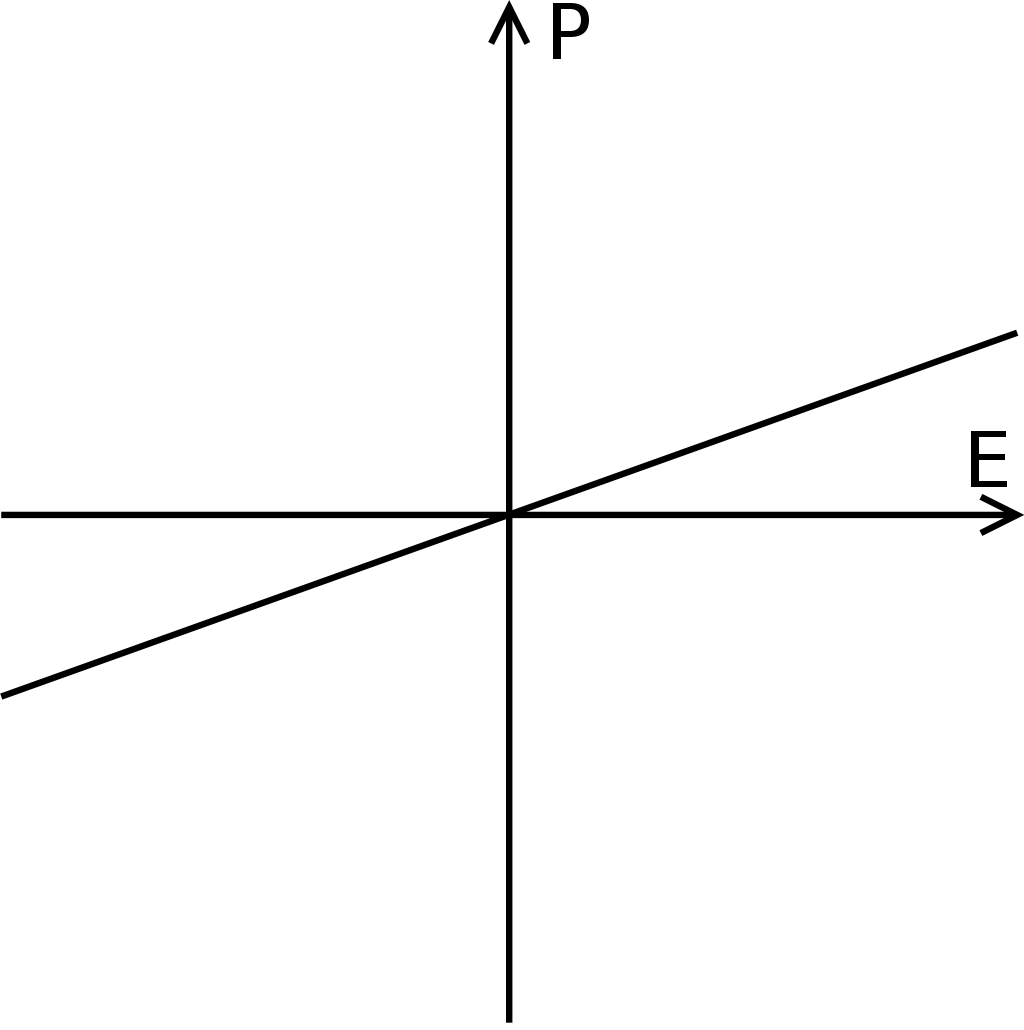
\includegraphics[scale=0.2]{dieletrico.png} 
\caption{Gráfico de $\vec{P}\times\vec{E}$ em dieletricos lineares.} 
\label{fig1} 
\end{figure}

Já para os materiais paraelétricos a polarização, embora dependa da aplicação de um campo elétrico externo para que o material se polarize, não possui uma relação totalmente linear como em (1). Um gráfico de $\vec{P}\times\vec{E}$ deste sistema está apresentado na Figura \ref{fig2}, nele é fácil observar essa não-linearidade.

\begin{figure}[H] 
\centering
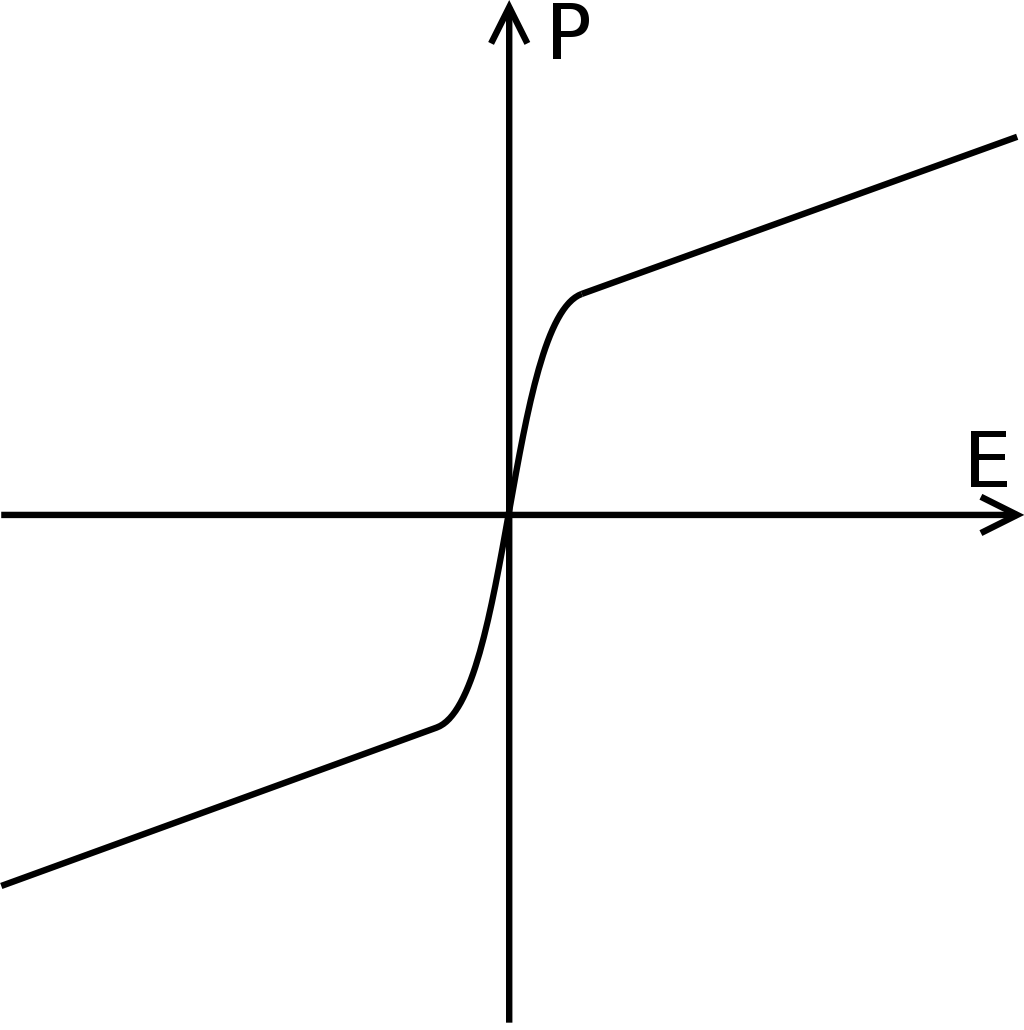
\includegraphics[scale=0.2]{paraeletrico.png} 
\caption{Gráfico de $\vec{P}\times\vec{E}$ em paraeletricos=.} 
\label{fig2} 
\end{figure}

Por fim, os materiais ferroelétricos possuem polarização espontânea diferente de zero, ao contrário dos dois anteriores, mas não é linear assim como o paraelétrico. Um gráfico de $\vec{P}\times\vec{E}$ deste tipo de material está apresentado na Figura \ref{fig3}.

\begin{figure}[H] 
\centering
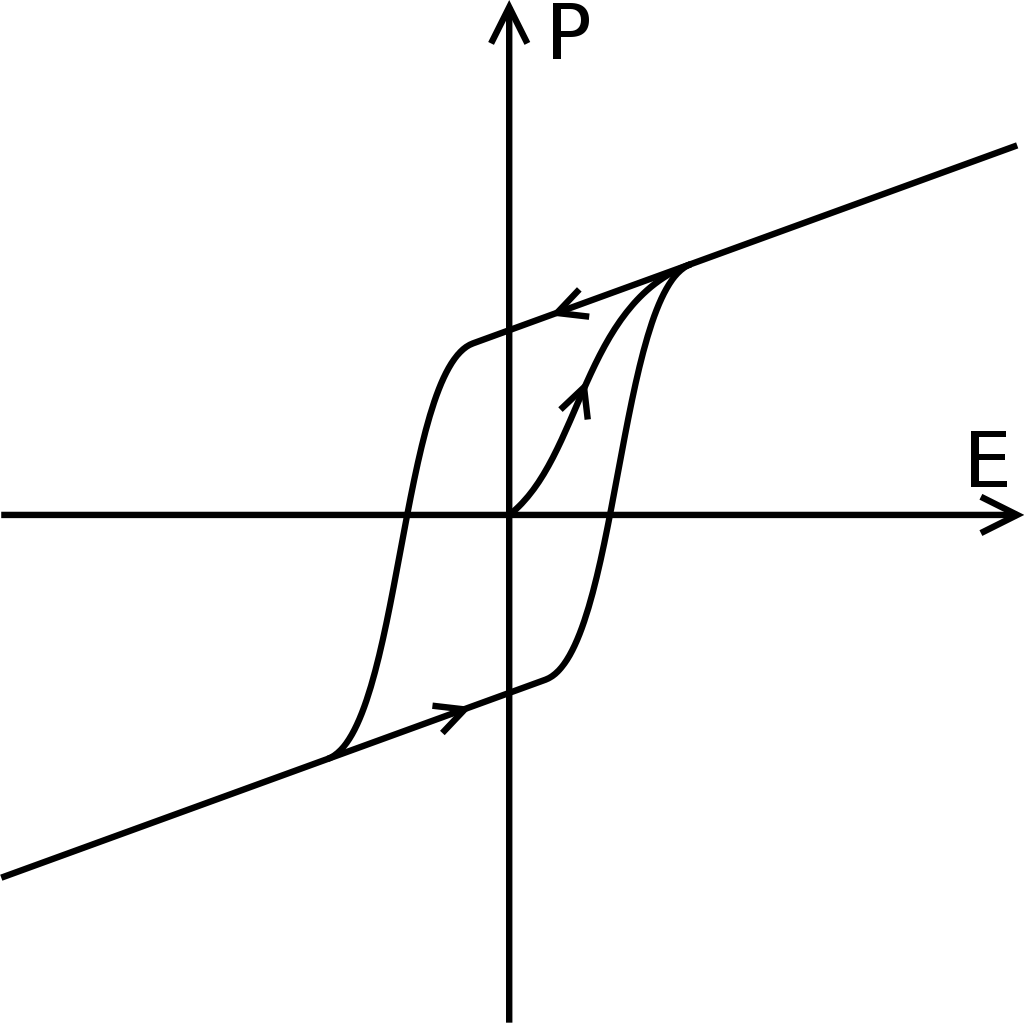
\includegraphics[scale=0.2]{ferroeletrico.png} 
\caption{Gráfico de $\vec{P}\times\vec{E}$ em ferroeletricos.} 
\label{fig3} 
\end{figure}

A quebra de simetria reside na dependência do comportamento destes materiais com a temperatura: podem apresentar-se como paraelétricos ou ferroelétricos. Neste caso, ele é ferroelétrico à temperaturas abaixo de $T_C$ e é paraelétrico acima dessa temperatura. Em outras palavras, a polarização espontânea desaparece ao ultrapassar tal temperatura, e o cristal ferroelétrico se transforma cristal paraelétrico (inclusive alterando sua estrutura cristalina [1]). Um fato que encontramos é que muitos ferroelétricos perdem suas propriedades acima de $T_C$ completamente, uma vez que a sua fase paraelétrica tem uma estrutura cristalina centrosimétrica [1]. Os gráficos que evidenciam essa quebra de simetria estão mostrados na Figura \ref{fig4}.

\begin{figure}[H] 
\centering
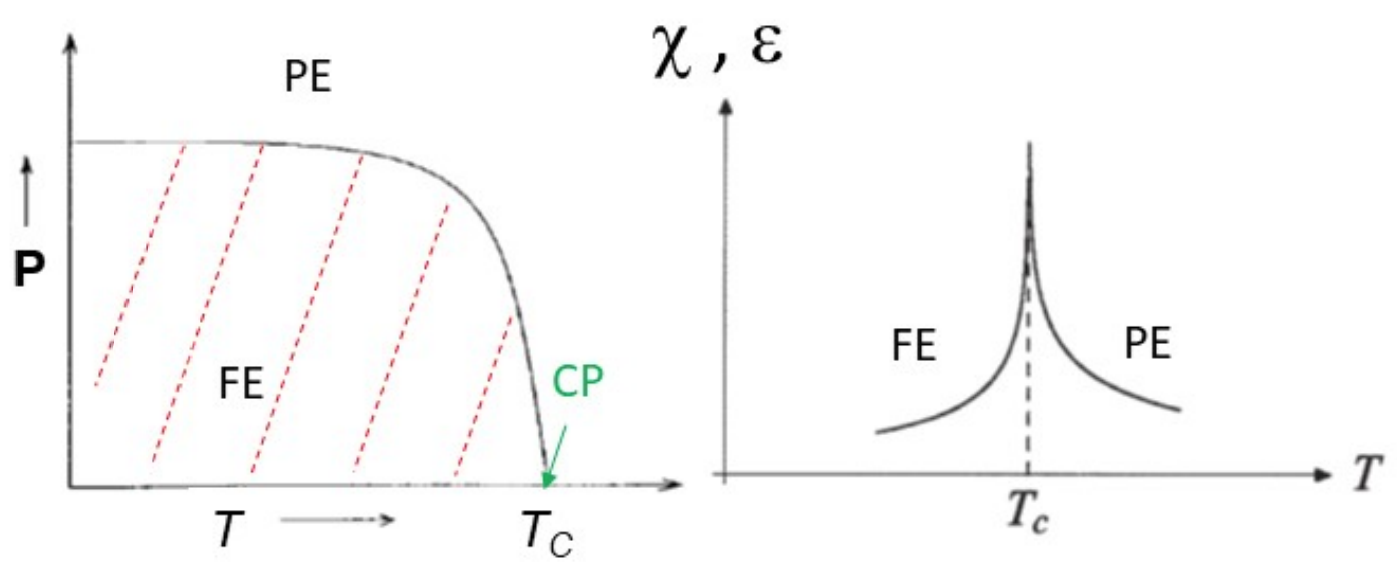
\includegraphics[scale=0.3]{quebradesimetria.png} 
\caption{Gráficos da quebra de simetria por $T_C$.} 
\label{fig4} 
\end{figure}

Quanto às condições de contorno, temos que quando $\lVert\vec{E}\rVert$ é muito grande, todos os três materiais apresentam comportamento linear, semelhante ao dielétrico. Por outro lado, quando $\lVert\vec{E}\rVert\sim 0$, enquanto materiais dielétricos e paraelétricos apresentam polarização nula, os materiais ferroelétricos apresentam polarização não nula.

\item Em [1], Trainer define a componente complexa de $\chi (T)$ como:
\eq\chi (T) = \chi' + i\chi''\feq
O valor de $\chi''$ é quantificado por meio da razão:
\eq\tg\delta = \dfrac{\chi''}{\chi'}\feq
onde $\tg{\delta}$ é a energia perdida por ciclo na forma de calor. Neste caso, $\chi'$ é obtido pelo valor da capacitância medida por meio da seguinte equação:
\eq C = \dfrac{Q}{V} = C_0(1+\chi')\feq
onde $C_0 = \epsilon_0A/d$.

Na Figura \ref{fig5} pode-se ver que o valor de $\chi''$ aumenta perto da transição de fase. Isso ocorre devido ao que chamamos de relaxamento dielétrico. Para um dielétrico é ideal que $\chi''$ seja pequeno, pois é necessária uma baixa perda de energia por ciclo. Em contrapartida, a alta perda de energia por ciclo causa o aquecimento do capacitor que, em determinadas circunstâncias, pode levar a uma quebra destrutiva do dielétrico.

\begin{figure}[H] 
\centering
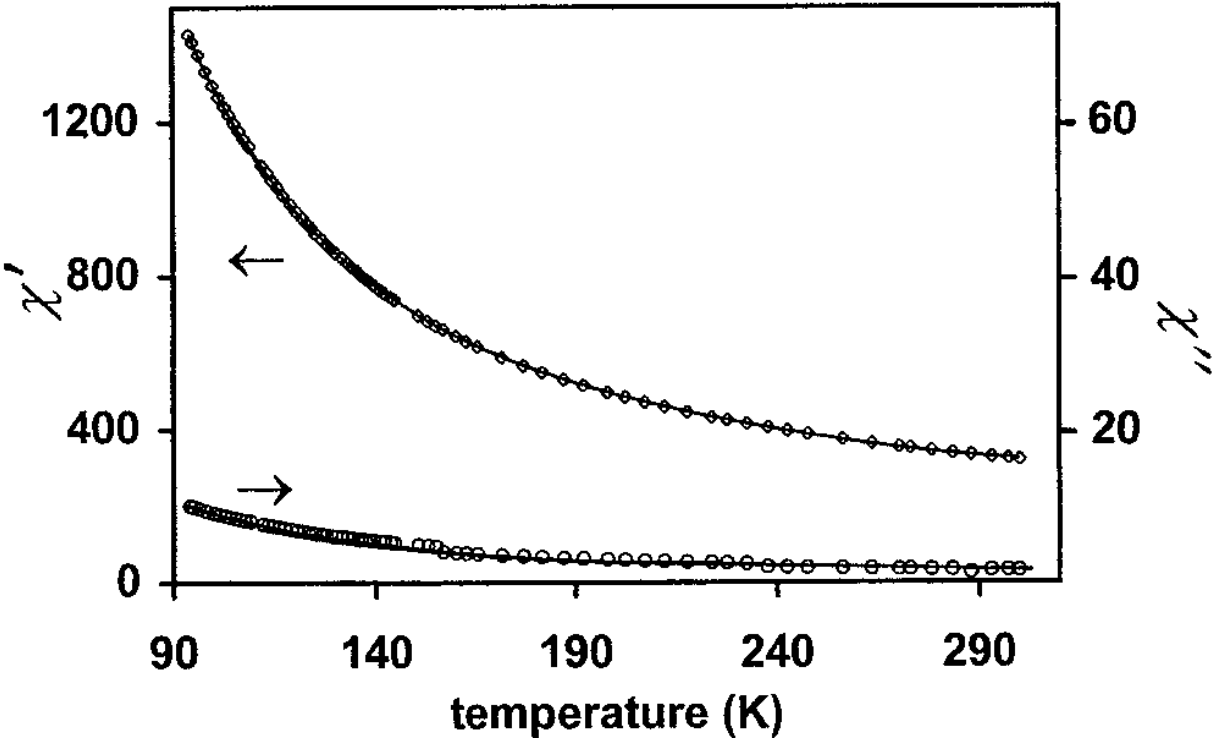
\includegraphics[scale=0.4]{suscetibilidadeeletrica.png} 
\caption{Gráfico de suscetibilidade elétrica do SrTiO$_3$ vs Temperatura.} 
\label{fig5} 
\end{figure}

\item 
No artigo do Trainer [1], verifica-se que o intervalo encontrado no qual vale a lei de Curie-Wiess corresponde a $110^oC<T<300^oC$. Esta lei é dada por:
\eq\chi_e = \dfrac{C_{CW}}{\left( T-T_0 \right)}\feq

Quanto ao comportamento do dos campos $\vec{E}$, $\vec{P}$ e $\vec{D}$, temos que $\vec{E}$ varia de maneira independente da temperatura do sistema, já que ele é um campo externo aplicado para a mudança de polarização do sistema. Dada a variação da temperatura e do campo elétrico, podemos encontrar o comportamento do campo de polarização a partir da equação (1) onde $\chi_e$ é dado pela lei de Curie Wiess (5), nos dando que:
\eq\vec{P} = \epsilon_0 \dfrac{C_{CW}}{\left( T-T_0 \right)} \vec{E}\feq

Onde $C_{CW}$ é a constante de Curie-Wiess, $T_0$ é a temperatura de Curie-Wiess e $T$ é a temperatura do sistema. Ao fixar uma determinada temperatura na equação (6), vemos que ela descreve uma relação linear entre a polarização e o campo elétrico, mas sabemos que a relação entre estes dois campos é, por definição, não linear. Dado isso, procuramos possíveis respostas para isso nos artigos do Case Study, no livro de eletrodinâmica do Griffths, do Reitz e de maneira muito mais ampla na internet, no entanto, não tivemos o sucesso de encontrar algum desenvolvimento satisfatório para esta questão. O mais perto que conseguimos chegar de um bom palpite é que isso pode ocorrer devido às flutuações quânticas explicadas pela mecânica quântica no artigo do Rowley [2].

Por fim, o campo de deslocamento elétrico, $\vec{D}$, que é relacionado com os outros dois pela expressão \eq\vec{D} = \left ( 1+ \chi_e \right ) \epsilon_0 \vec{E}\feq

Substituindo novamente $\chi_e$ pela lei de Curie-Wiess, chegamos a:
\eq\vec{D} = \left ( 1+ \dfrac{C_{CW}}{\left( T-T_0 \right)}\right) \epsilon_0 \vec{E}\feq

Dado que o material deve se comportar como ferroelétrico quando $T<T_0$ se como paraelétrico quando  $T>T_0$, temos que o gráfico de $\vec{P} \times \vec{E}$ deles serão a Figura \ref{fig3} e a Figura \ref{fig2}, respectivamente.

\item Pelo artigo de Rowley [2], vimos que, quando a fronteira entre a paraeletricidade e a ferroeletricidade se encontra em baixas temperaturas, elas são mais sutis e complexas do que o que foi previsto pela eletrodinâmica clássica. Neste artigo, por exemplo, é apresentado o comportamento de vários materiais na fronteira da ferroeletricidade, observando assim dependências não-clássicas da temperatura $T$ da  função dielétrica inversa $1/\epsilon $ abaixo de 50K, além elevações anormais em temperaturas menores, estendendo-se até a faixa de milikelvins. Tal comportamento anômalo é evidenciado ao observar a Figura \ref{fig6} e a Figura \ref{fig7}.

\begin{figure}[H] 
\centering
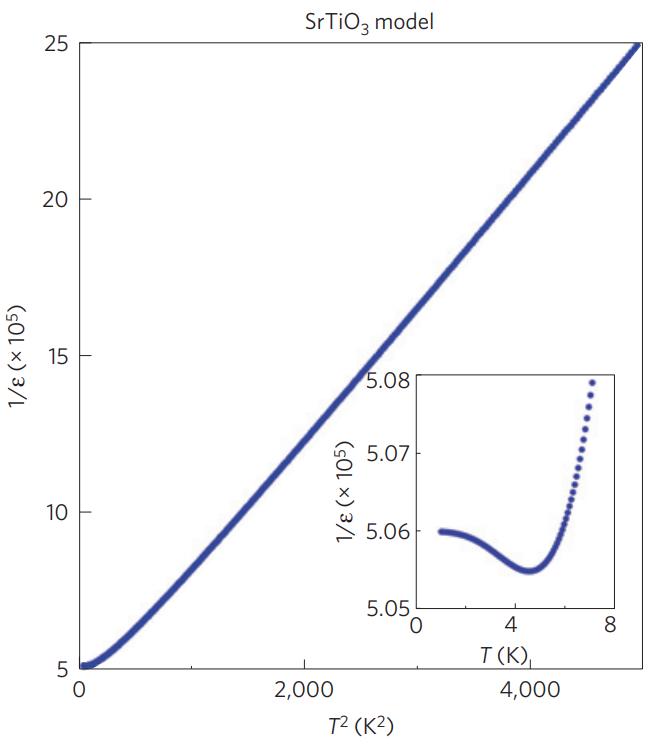
\includegraphics[scale=0.6]{srtio.png} 
\caption{Gráfico de $1/\epsilon\times T^2$ do SrTiO$_3$.} 
\label{fig6} 
\end{figure}

\begin{figure}[H] 
\centering
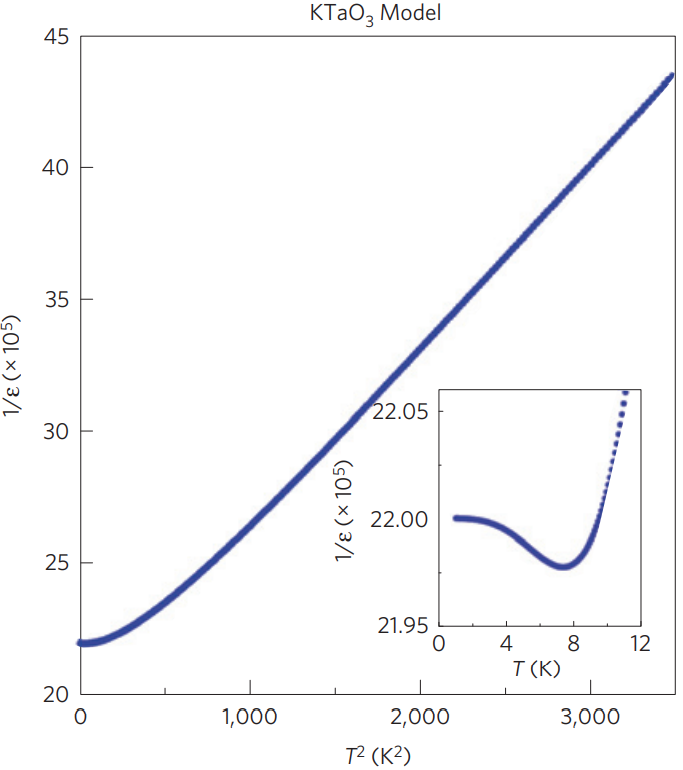
\includegraphics[scale=0.6]{ktao.png} 
\caption{Gráfico de $1/\epsilon\times T^2$ do KTaO$_3$.} 
\label{fig7} 
\end{figure}

Com o nosso conhecimento de eletrodinâmica, concordamos com a interpretação de Rowley quando ele desconsidera a polarização $\vec{P}$ como um parâmetro de ordem para descrever a física subjacente do ponto crítico quântico ferroelétrico ($T_C = 0$ K), uma vez que fenômenos decorrentes de flutuações quânticas passam a se tornar muito mais relevantes em temperaturas próximas a esta. Tanto na Figura \ref{fig6} como na Figura \ref{fig7}, observa-se que há linearidade apenas para temperaturas muito maiores que $T_C$, como previsto pela eletrodinâmica clássica.

Os materiais ferroelétricos descritos por ele no artigo exibem transições entre estados homogêneos sem a aplicação de campos de quebra de simetria e não envolvem a complicação de redução dimensional. A dimensão efetiva na descrição do ponto crítico do quântica é de forma surpreendente a dimensão marginal de $3+1$, ou seja, três dimensões de espaço mais uma dimensão de tempo como é o caso da física de partículas elementares. Ao considerar $d_{eff} = 4$, Rowley obtém um valor para a suscetibilidade elétrica proporcional a $1/T^2$, o qual induz excitações de energia de baixa altitude. Portanto, também concordamos com ele ao fazer tal afirmação, que dispensa o uso da termodinâmica nestas escalas.

\item Existem inúmeras aplicações decorrentes deste estudo pois, com a compreensão do comportamento dos materiais ferroelétricos em baixas temperaturas, será possível por exemplo ser feito filmes (de supercondutores) com apenas 1 nanômetro de espessura, o que significa que essas células de armazenamento podem ser reduzidas a dimensões abaixo do que acreditavamos ser possível.

\end{enumerate}
\section{Conclusão}
Por fim, ficou claro que o estudo dos fênomenos de polarização na matéria não tem suas respostas apenas no eletromagnetismo, mas também na termodinamica e na mecânica quântica. Este último em particular trás um novo horizonte ainda inesplorado pelos limites das outras duas. O estudo de caso no geral foi fundamental para a nossa compreensão de como os conceitos vistos em aula refletem na prática, já com o auxílio e correções de outras áreas da Física.

\section{Bibliografia}
[1] Trainer, Matthew (2001) - \textit{Ferroelectricity: Measurement of the dielectric susceptibility
of strontium titanate at low temperatures} \\

[2] Rowley, S.E (2014) - \textit{Ferroelectric quantum criticality} \\

[3] Safari, Ahmad (2008) - \textit{Piezoelectric and acoustic materials for transducer applications.}

\end{document}
